\section{Problem formulation and analysis}
\noindent We would like to formalize the formulation of Hoffman's multidimensional packing problem. Let $n$ be a positive integer denoting the dimension of the problem. We will refer to an element $d$ of $(0, \infty)^n$ as an $n$-dimensional \textit{dimension tuple}\index{Dimension tuple} and we refer to the sum of its coordinates as the sum of the dimension tuple\index{Dimension tuple!sum of}. Note that we will typically omit the ``$n$-dimensional'' part of notions, whenever it is clear from the context and for instance simply write ``dimension tuple''.

\begin{definition}[Hyperrectangle]\index{Hyperrectangle}
A subset $R$ of $\R^n$ is an $n$-dimensional \textit{hyperrectangle}, if it can be written as a Cartesian product of $n$ non-empty, open and bounded intervals $I_1, I_2, \dotsc, I_n$ of $\R$, that is $R = I_1 \times I_2 \times \dotsb \times I_n$.
\end{definition}

\noindent In addition, for each $i = 1, 2, \dotsc, n$ let $a_i$ and $b_i$ denote the left and right endpoints of the interval $I_i = (a_i, b_i)$, let $x_i = b_i - a_i$ denote the interval width and let $m_i = (a_i + b_i)/2$ denote the interval midpoint. We will refer to the point $\paren{a_1, a_2, \dotsc, a_n}$ as the \textit{anchor point}\index{Hyperrectangle!anchor point of} and the point $\paren{m_1, m_2, \dotsc, m_n}$ as the \textit{centre}\index{Hyperrectangle!centre of} of the hyperrectangle $R$. We will refer to the tuple $\paren{x_1, x_2, \dotsc, x_n}$ as the dimension tuple of the hyperrectangle\index{Hyperrectangle!dimension tuple of} $R$ and refer to its $i$'th element as the \textit{extent}\index{Hyperrectangle!extend of} of the hyperrectangle along the $i$'th dimension. Lastly, the $n$-dimensional \textit{hypervolume}\index{Hyperrectangle!hypervolume of} of the hyperrectangle $R$ is the product $x_1 x_2 \dotsm x_n$.

Notice that the hyperrectangle $R$ is uniquely identified by its anchor point and dimension tuple, since this information determines the endpoints of $I_i$ for each $i = 1, 2, \dotsc, n$. When we are not interested in the ``position'' of a hyperrectangle in $\R^n$, we will typically just refer to it by its dimension tuple.

\begin{definition}[Hypercube]\index{Hypercube}
An $n$-dimensional \textit{hypercube} is an $n$-dimensional hyperrectangle with the same extent along all dimensions, i.e.\ $x_1 = x_2 = \dotsb = x_n$.
\end{definition}

\begin{definition}[General hyperrectangle]\index{Hyperrectangle!general}
A subset of $\R^n$ is an $n$-dimensional \textit{general hyperrectangle} if it can be rotated into an $n$-dimensional hyperrectangle.
\end{definition}

\noindent Two general hyperrectangles are said to be \textit{overlapping}\index{Hyperrectangle!overlapping} if they intersect one another and \textit{non-overlapping}\index{Hyperrectangle!non-overlapping} if they are disjoint.

\begin{definition}[Packing]\label[definition]{def:general-packing}\index{Packing}
Let $d$ be an $n$-dimensional dimension tuple and let $s$ denote its sum. Suppose $C$ is an $n$-dimensional hypercube with extent $s$, and suppose $B$ is a set of $n$-dimensional general hyperrectangles of $\R^n$, all of which can be rotated into an $n$-dimensional hyperrectangle with dimension tuple $d$. Then $\paren{B, C}$ is a \textit{packing} of $d$, if
\begin{enumerate}[(i)]
  \item The general hyperrectangles in $B$ are pairwise non-overlapping.
  \item Each general hyperrectangle in $B$ is contained in $C$.
\end{enumerate}
\end{definition}

\noindent We will refer to $C$ as the \textit{surrounding}\index{Hypercube!surrounding} hypercube. Note that we can always translate the general hyperrectangles in $B$ and the surrounding hypercube $C$ of a packing $(B, C)$, so that the surrounding hypercube has its centre at the origin of the coordinate system. From now on we will assume that such a translation has been performed, unless otherwise stated. We are now ready to formulate the $n$-dimensional packing problem.

\begin{definition}[Good dimension]
A positive integer $n$ is a good dimension, if for any choice of $n$-dimensional dimension tuple $d$ there exists a packing of $d$.
\end{definition}

\noindent Hoffman asks the following question in \cite[p. 222]{Hoffman1981}, which according to \cite[p. 914]{berlekamp_conway_guy_2004} and recent correspondences with Dean G. Hoffman \cite{hoffman_private} does not appear to have been answered for all dimensions.

\begin{question}
For which positive integers $n$, is $n$ a good dimension?
\end{question}

\noindent \cref{fig:universal-packing-2d} demonstrates that $2$ is a good dimension by showing how to construct a packing of any two-dimensional dimension tuple. According to \cite[p. 215]{Hoffman1981} $3$ is good, but Hoffman does not provide a thorough proof. We provide the first thorough proof of this in \cref{thm:three-is-good}. \cref{thm:multiplication-of-packings} below shows that this packing problem exhibits an extraordinary property, which in particular implies that the number of good dimensions is unbounded. The first appearance of this result is unclear, but Hoffman attributes it to Raphael Robinson in \cite[p. 223]{Hoffman1981}, while Elwyn R. Berlekamp et al. \cite[p. 914]{berlekamp_conway_guy_2004} attribute it to David Seal as well. The proof is based on the one presented by Hoffman in \cite[p. 223--225]{Hoffman1981}.

\FloatBarrier
\begin{theorem}\label[theorem]{thm:multiplication-of-packings}
Suppose $m$ and $n$ are positive integers. If both $m$ and $n$ are good dimensions, then $mn$ is a good dimension as well.
\end{theorem}
\begin{proof}
Suppose $m$ and $n$ are good dimensions and let
\[
\paren{
x_{1, 1}, x_{1, 2}, \dotsc, x_{1, n},
x_{2, 1}, x_{2, 2}, \dotsc, x_{2, n},
\dotsc,
x_{m, 1}, x_{m, 2}, \dotsc, x_{m, n}
}
\]
be an $mn$-dimensional dimension tuple and let $t$ denote its sum. We would like to show that there exists a packing of this dimension tuple. Suppose we have $(mn)^{mn}$ $mn$-dimensional hyperrectangles with the above dimension tuple. We would like to rotate and translate them to fit inside an $mn$-dimensional hypercube with an extent of $t$. For the sake of readability we will write out the dimension tuple in an $m \times n$ matrix
\[
A = \begin{pmatrix}
x_{1, 1} & x_{1, 2} & \cdots & x_{1, n} \\
x_{2, 1} & x_{2, 2} & \cdots & x_{2, n} \\
\vdots   & \vdots   & \ddots & \vdots   \\
x_{m, 1} & x_{m, 2} & \cdots & x_{m, n}
\end{pmatrix}.
\]
Let $s_i$ be the sum of the $i$'th column of $A$ for $i = 1, 2, \dotsc, n$. First, divide the $(mn)^{mn}$ $mn$-dimensional hyperrectangles into groups, each consisting of $m^m$ hyperrectangles. There must be $(mn)^{mn}/m^m = m^{m(n-1)}n^{mn}$ of these groups. Consider the dimension tuple $\paren{x_{1, 1}, x_{2, 1}, \dotsc, x_{m, 1}}$ consisting of the first column of $A$ and recall that its sum is $s_1$. Since $m$ is a good dimension, there exists a packing of $m^m$ $m$-dimensional general hyperrectangles (which can be rotated to have this dimension tuple) inside an $m$-dimensional hypercube with an extent of $s_1$. Then we see that the $m^m$ $mn$-dimensional hyperrectangles in each group will fit inside an $mn$-dimensional hyperrectangle with dimension tuple (as a matrix)
\[
\begin{pmatrix}
s_1    & x_{1, 2} & \cdots & x_{1, n} \\
s_1    & x_{2, 2} & \cdots & x_{2, n} \\
\vdots & \vdots   & \ddots & \vdots   \\
s_1    & x_{m, 2} & \cdots & x_{m, n}
\end{pmatrix}.
\]
By ``fit'' we mean that the $m^m$ hyperrectangles are pairwise non-overlapping and rotated and translated such that they are subsets of the surrounding hyperrectangle like in \cref{def:general-packing}. Doing this for each group results in $m^{m(n-1)}n^{mn}$ such $mn$-dimensional hyperrectangles---each containing $m^m$ of the original $mn$-dimensional hyperrectangles, rotated and translated appropriately. We repeat this procedure for every column, each time dividing the $mn$-dimensional hyperrectangles constructed at the previous iteration into groups with a size of $m^m$ and then fitting the hyperrectangles of each group into a surrounding $mn$-dimensional hyperrectangle. After doing this a total number of $n$ times, we end up with $n^{mn}$ groups of $mn$-dimensional hyperrectangles each of which fits inside an $mn$-dimensional hyperrectangle with dimension tuple (as a matrix)
\[
B = \begin{pmatrix}
s_1    & s_2    & \cdots & s_n    \\
s_1    & s_2    & \cdots & s_n    \\
\vdots & \vdots & \ddots & \vdots \\
s_1    & s_2    & \cdots & s_n
\end{pmatrix}.
\]
Each of these $mn$-dimensional hyperrectangles contains $m^{mn}$ of the original $mn$-dimensional hyperrectangles, rotated and translated appropriately. Next, we perform a similar procedure for each row. We divide the $n^{mn}$ $mn$-dimensional hyperrectangles into groups of $n^n$ hyperrectangles. There are $n^{mn}/n^n = n^{(m - 1)n}$ of these groups. Consider the dimension tuple $\paren{s_1, s_2, \dotsc, s_n}$ consisting of the first row of $B$ and notice that the sum along this row is $t$. Since $n$ is a good dimension, there exists a packing of $n^n$ $n$-dimensional general hyperrectangles (which can be rotated to have this dimension tuple) inside an $n$-dimensional hypercube with an extent of $t$. Then the $n^n$ $mn$-dimensional hyperrectangles in each group will fit inside an $mn$-dimensional hyperrectangle with dimension tuple (as a matrix)
\[
\begin{pmatrix}
t      & t      & \cdots & t      \\
s_1    & s_2    & \cdots & s_n    \\
\vdots & \vdots & \ddots & \vdots \\
s_1    & s_2    & \cdots & s_n
\end{pmatrix}.
\]
Doing so for each group, we obtain $n^{(m - 1)n}$ such $mn$-dimensional hyperrectangles---each containing $m^{mn} n^n$ of the original $mn$-dimensional hyperrectangles, rotated and translated appropriately. Repeating this procedure for each row, $m$ times in total, we end up with $n^{(m - m)n} = 1$ group of $n^n$ $mn$-dimensional hyperrectangles fitting inside an $mn$-dimensional hyperrectangle with dimension tuple (as a matrix)
\[
\begin{pmatrix}
t      & t      & \cdots & t      \\
t      & t      & \cdots & t      \\
\vdots & \vdots & \ddots & \vdots \\
t      & t      & \cdots & t
\end{pmatrix}.
\]
This is in fact an $mn$-dimensional hypercube with an extent of $t$ and the desired packing is obtained by repeatedly unwrapping the groups of rotated and translated $mn$-dimensional hyperrectangles, until we reach the now appropriately rotated and translated $(mn)^{mn}$ $mn$-dimensional hyperrectangles.
\end{proof}

\noindent It follows from this result that in order to prove that all dimensions are good, one would only have to prove so for all prime numbers. Hence, 4 is a good dimension, and in the light of \cref{thm:three-is-good} the smallest unsettled dimension is 5 \cite[p. 223]{Hoffman1981}\cite[p. 914]{berlekamp_conway_guy_2004}.

If $n$ is a good dimension, it is natural to ask how many different packings there are in that particular dimension. Before we can even attempt to answer this question, we need to make sure that the number of different packings is independent of the choice of dimension tuple. This will ultimately lead to the definition of a universal packing and a refinement of the question. In preparation for this, we will first need a notion of two packings being notably different.

\subsection{Equivalence of packings}
Depending on the choice of dimension tuple $d$ there might be enough unoccupied ``room'' inside the surrounding hypercube to rearrange the general hyperrectangles without intersecting one another and without leaving the surrounding hypercube.

\begin{definition}[Rearrangement]\index{Packing!rearrangement of}
Suppose $(B_1, C_1)$ and $(B_2, C_2)$ are packings of the dimension tuples $d_1$ and $d_2$, respectively. The first packing is a \textit{rearrangement} of the second if $C_1$ coincides with $C_2$ and if it is possible to continuously move (using only translations and rotations) the general hyperrectangles in $B_1$, so that each moved general hyperrectangle coincides with a general hyperrectangle in $B_2$ without breaking any of the criteria in \cref{def:general-packing} while moving.
\end{definition}

\begin{figure}[h]
    \centering
    \begin{subfigure}[b]{0.37\textwidth}
        \centering
            \begin{tikzpicture}[scale=0.60*5/3]
                \draw (0, 0) rectangle (3, 3);
                \filldraw[fill=custom-red, draw=black] (0, 0) rectangle (1, 2);
                \filldraw[fill=custom-red, draw=black] (1, 0) rectangle (2, 2);
                \filldraw[fill=custom-red, draw=black] (2, 0) rectangle (3, 2);
                \filldraw[fill=custom-red, draw=black] (0, 2) rectangle (2, 3);
                \draw[decorate,decoration={brace, raise=2pt, amplitude=4pt}] (0, 2)  -- node[midway, left=3pt]{$x_1$} (0, 3);
                \draw[decorate,decoration={brace, raise=2pt, amplitude=4pt}] (0, 3)  -- node[midway, above=3pt]{$x_2$} (2, 3);
            \end{tikzpicture}
        \caption{Packing with three rectangles side by side.}
        \label{fig:extreme-packing-2d}
    \end{subfigure}
    ~
    \begin{subfigure}[b]{0.37\textwidth}
        \centering
            \begin{tikzpicture}[scale=0.60*5/3]
                \draw (0, 0) rectangle (3, 3);
                \filldraw[fill=custom-red, draw=black] (0, 0) rectangle (1, 2);
                \filldraw[fill=custom-red, draw=black] (1, 0) rectangle (2, 2);
                \filldraw[fill=custom-red, draw=black] (2, 1) rectangle (3, 3);
                \filldraw[fill=custom-red, draw=black] (0, 2) rectangle (2, 3);
                \draw[decorate,decoration={brace, raise=2pt, amplitude=4pt}] (0, 2)  -- node[midway, left=3pt]{$x_1$} (0, 3);
                \draw[decorate,decoration={brace, raise=2pt, amplitude=4pt}] (0, 3)  -- node[midway, above=3pt]{$x_2$} (2, 3);
            \end{tikzpicture}
        \caption{Rearrangement of the packing in Figure \ref{fig:extreme-packing-2d}.}
        \label{fig:rearrangement-packing-2d}
    \end{subfigure}
    \caption{Example of equivalent two-dimensional packings of the dimension tuple $\paren{x_1, x_2}$ where $x_2 = 2 x_1$.}
\end{figure}

\noindent It is also natural to take reflections and rotations of the packing as a whole into account. We can view such a transformation as a linear map represented by an orthogonal $n \times n$ matrix. There are an infinite number of these, but by \cref{def:general-packing} we only have to consider those mapping the surrounding hypercube to itself. This corresponds to the linear maps sending the standard basis vectors $e_1, e_2, \dotsc, e_n$ to some permutation of themselves while possibly changing the sign of some of them. Thus, there are $n! \cdot 2^n$ reflections and/or rotations of an $n$-dimensional hypercube. We will refer to reflections and/or rotations as \textit{symmetries}\index{Packing!symmetry of}. With this in mind, we will define what it means for two packings to be equivalent.

\begin{definition}[Equivalent packings]\index{Packing!equivalence of}
Suppose there are two packings of the dimension tuples $d_1$ and $d_2$, respectively. These packings are \textit{equivalent} if there exists a rearrangement of the first packing coinciding with a symmetry of the second.
\end{definition}

\noindent This is an equivalence relation and we will refer to the equivalence classes as unique packings. Notice that it is possible to permute the elements in a dimension tuple without influencing the number of unique packings, since such a permutation corresponds to rotating all packings and thus does not affect the equivalence classes. We can therefore without loss of generality restrict ourselves to increasing dimension tuples. We say that a dimension tuple $d = \paren{x_1, x_2, \dotsc, x_n}$ is \textit{increasing}\index{Dimension tuple!increasing} if $x_1 \leq x_2 \leq \dotsb \leq x_n$.

The notion of rearrangements of a packing also gives rise to defining a rigid packing, that is a packing where all the general hyperrectangles are ``locked into place'' by the surrounding general hyperrectangles or hypercube.

\begin{definition}[Rigid packing]\index{Packing!rigid}
We say that a packing is \textit{rigid} if all of its rearrangements are identical to itself.
\end{definition}

\noindent \cref{fig:universal-packing-2d} is an example of a rigid packing. Note that the equivalence class of a rigid packing only contains its symmetries, so it contains at most $n! \cdot 2^n$ packings. It might contain fewer if some symmetries are identical to one another.

Next, we will examine packings of dimension tuples satisfying a certain inequality, which forces any packing consisting of hyperrectangles to be rigid and ultimately leads to the definition of a universal packing.

\subsection{Universal packings} Before defining a universal packing, it is helpful to get some intuition by looking a bit closer at the two-dimensional packing problem. Consider some increasing dimension tuple $\paren{x_1, x_2}$. There are ways of organizing the four rectangles, which are only possible when the relative difference between $x_1$ and $x_2$ is sufficiently large. Suppose $x_2$ is twice as large as $x_1$, i.e.\ $x_2 = 2x_1$ or equivalently $x_1 + x_2 = 3 x_1$. Then the packing in Figure \ref{fig:extreme-packing-2d} becomes possible. This packing is only feasible because we can fit three rectangles side by side. It turns out that restricting the search to packings of increasing dimension tuples satisfying the inequality
\begin{equation}\label{eq:ineq-2d}
x_1 + x_2 < 3x_1
\end{equation}
prevents this and restricts the problem in an interesting way. Later, we will argue that any packing of an increasing dimension tuple satisfying \eqref{eq:ineq-2d} consisting of hyperrectangles will be rigid and discuss whether it gives a ``recipe'' for constructing a packing of \textit{any} dimension tuple as seen in \cref{fig:universal-packing-2d}. Thus, it is possible to reuse the same ``universal packing'' even for dimension tuples not satisfying \eqref{eq:ineq-2d}. This is the inspiration behind our future definition of a ``universal packing''.

Notice that the packing in \cref{fig:extreme-packing-2d}---which relied on \eqref{eq:ineq-2d} not being satisfied---is not rigid. Intuitively, \eqref{eq:ineq-2d} ensures that the four rectangles resemble a square to such a degree that any packing must necessarily resemble the packing \cref{fig:2d-packing-squares}, where four squares are neatly organized in a grid inside the surrounding square. We will return to this concept of a grid shortly. The inequality \eqref{eq:ineq-2d} is inspired by Hoffman who proposed a three-dimensional version of it in \cite[p. 215]{Hoffman1981}, namely
\begin{equation}\label{eq:ineq-3d}
x_1 + x_2 + x_3 < 4x_1.
\end{equation}
Therefore we will name it after Hoffman when we generalize it to $n$ dimensions.

\begin{definition}[Hoffman's inequality]\index{Hoffman's inequality}
A dimension tuple $\paren{x_1, x_2, \dotsc, x_n}$ satisfies \textit{Hoffman's inequality} if it is increasing and
\[
x_1 + x_2 + \dotsb + x_n < (n + 1)x_1.
\]
\end{definition}

\noindent Choosing $x_1 = x_2 = \dotsb = x_n$ for some positive real number shows that a dimension tuple with this property exists in all dimensions. Notice that \eqref{eq:ineq-2d} and \eqref{eq:ineq-3d} are really Hoffman's inequality for $n = 2$ and $n = 3$, respectively. Intuitively, Hoffman's inequality ensures that no packing can contain $n + 1$ or more hyperrectangles side by side. Shortly, we will justify that packings (consisting solely of hyperrectangles) of a dimension tuple satisfying Hoffman's inequality must be rigid and prove that the hyperrectangles must be arranged in a ``grid''.

Hoffman restricts his search for three-dimensional packings in \cite[p. 215]{Hoffman1981} to dimension tuples satisfying Hoffman's inequality for $n = 3$, that is \eqref{eq:ineq-3d}. George Miller \cite{Miller_2006} credits Donald Knuth for searching for three-dimensional packings of the dimension tuple $\paren{3, 4, 5}$ and discovering solutions where one could squeeze an additional 28th 3-dimensional hyperrectangle (brick) into the surrounding cube (which has an extent of $3 + 4 + 5 = 12$).
\begin{figure}[ht]
    \centering
    \begin{subfigure}[b]{0.8\textwidth}
        \centering
            \begin{tikzpicture}[scale=0.2*15/12]
            \filldraw[fill=custom-green, draw=black] (0,0) rectangle (3,5);
\filldraw[fill=custom-green, draw=black] (3,0) rectangle (6,5);
\filldraw[fill=custom-green, draw=black] (6,0) rectangle (9,5);
\filldraw[fill=custom-green, draw=black] (9,0) rectangle (12,5);

\filldraw[fill=custom-red, draw=black] (0,5) rectangle (4,9);
\filldraw[fill=custom-red, draw=black] (4,5) rectangle (8,9);
\filldraw[fill=custom-red, draw=black] (8,5) rectangle (12,9);

\filldraw[fill=custom-red, draw=black] (0,8) rectangle (3,12);
\filldraw[fill=custom-red, draw=black] (3,8) rectangle (6,12);
\filldraw[fill=custom-red, draw=black] (6,8) rectangle (9,12);
\filldraw[fill=custom-red, draw=black] (9,8) rectangle (12,12);

            \end{tikzpicture}
            \hfill
            \begin{tikzpicture}[scale=0.2*15/12]
            \draw (0,0) rectangle (12,12);

\filldraw[fill=custom-blue, draw=black] (0,0) rectangle (4,5);
\filldraw[fill=custom-blue, draw=black] (4,0) rectangle (8,5);
\filldraw[fill=custom-blue, draw=black] (8,0) rectangle (12,5);

\filldraw[fill=custom-blue, draw=black] (0,7) rectangle (4,12);
\filldraw[fill=custom-blue, draw=black] (4,7) rectangle (8,12);
\filldraw[fill=custom-blue, draw=black] (8,7) rectangle (12,12);

            \end{tikzpicture}
            \hfill
            \begin{tikzpicture}[scale=0.2*15/12]
            \filldraw[fill=custom-red, draw=black] (0,0) rectangle (4,4);
\filldraw[fill=custom-red, draw=black] (4,0) rectangle (8,4);
\filldraw[fill=custom-red, draw=black] (8,0) rectangle (12,4);

\filldraw[fill=custom-red, draw=black] (0,3) rectangle (3,7);
\filldraw[fill=custom-red, draw=black] (3,3) rectangle (6,7);
\filldraw[fill=custom-red, draw=black] (6,3) rectangle (9,7);
\filldraw[fill=custom-red, draw=black] (9,3) rectangle (12,7);

\filldraw[fill=custom-green, draw=black] (0,7) rectangle (3,12);
\filldraw[fill=custom-green, draw=black] (3,7) rectangle (6,12);
\filldraw[fill=custom-green, draw=black] (6,7) rectangle (9,12);
\filldraw[fill=custom-green, draw=black] (9,7) rectangle (12,12);

            \end{tikzpicture}
        \caption{Layers of first solution.}
    \end{subfigure}
    \par\bigskip
    \begin{subfigure}[b]{0.8\textwidth}
        \centering
            \begin{tikzpicture}[scale=0.2*15/12]
            \filldraw[fill=custom-red, draw=black] (0,8) rectangle (3,12);
\filldraw[fill=custom-red, draw=black] (3,8) rectangle (6,12);
\filldraw[fill=custom-red, draw=black] (6,8) rectangle (9,12);
\filldraw[fill=custom-red, draw=black] (9,8) rectangle (12,12);

\filldraw[fill=custom-red, draw=black] (0,4) rectangle (3,8);
\filldraw[fill=custom-red, draw=black] (3,4) rectangle (6,8);
\filldraw[fill=custom-red, draw=black] (6,4) rectangle (9,8);
\filldraw[fill=custom-red, draw=black] (9,4) rectangle (12,8);

\filldraw[fill=custom-red, draw=black] (0,0) rectangle (3,4);
\filldraw[fill=custom-red, draw=black] (3,0) rectangle (6,4);
\filldraw[fill=custom-red, draw=black] (6,0) rectangle (9,4);
\filldraw[fill=custom-red, draw=black] (9,0) rectangle (12,4);

            \end{tikzpicture}
            \hfill
            \begin{tikzpicture}[scale=0.2*15/12]
            \filldraw[fill=custom-green, draw=black] (0,0) rectangle (5,3);
\filldraw[fill=custom-blue, draw=black] (5,0) rectangle (9,5);
\filldraw[fill=custom-green, draw=black] (9,0) rectangle (12,5);

\filldraw[fill=custom-blue, draw=black] (0,3) rectangle (5,7);
\filldraw[fill=custom-blue, draw=black] (7,5) rectangle (12,9);

\filldraw[fill=custom-green, draw=black] (0,7) rectangle (3,12);
\filldraw[fill=custom-blue, draw=black] (3,7) rectangle (7,12);
\filldraw[fill=custom-green, draw=black] (7,9) rectangle (12,12);

            \end{tikzpicture}
            \hfill
            \begin{tikzpicture}[scale=0.2*15/12]
            \filldraw[fill=custom-blue, draw=black] (0,0) rectangle (5,4);
\filldraw[fill=custom-green, draw=black] (5,0) rectangle (8,5);
\filldraw[fill=custom-blue, draw=black] (8,0) rectangle (12,5);

\filldraw[fill=custom-green, draw=black] (0,4) rectangle (5,7);
\filldraw[fill=custom-green, draw=black] (7,5) rectangle (12,8);

\filldraw[fill=custom-blue, draw=black] (0,7) rectangle (4,12);
\filldraw[fill=custom-green, draw=black] (4,7) rectangle (7,12);
\filldraw[fill=custom-blue, draw=black] (7,8) rectangle (12,12);
            \end{tikzpicture}
        \caption{Layers of second solution.}
    \end{subfigure}
    \par\bigskip
    \begin{subfigure}[b]{0.8\textwidth}
        \centering
            \begin{tikzpicture}[scale=0.2*15/12]
            \filldraw[fill=custom-green, draw=black] (0,0) rectangle (5,3);
\filldraw[fill=custom-green, draw=black] (0,3) rectangle (5,6);
\filldraw[fill=custom-green, draw=black] (0,6) rectangle (5,9);
\filldraw[fill=custom-green, draw=black] (0,9) rectangle (5,12);

\filldraw[fill=custom-red, draw=black] (5,0) rectangle (9,3);
\filldraw[fill=custom-red, draw=black] (9,0) rectangle (12,4);
\filldraw[fill=custom-red, draw=black] (5,3) rectangle (8,7);
\filldraw[fill=custom-red, draw=black] (8,4) rectangle (12,7);

\filldraw[fill=custom-blue, draw=black] (5,7) rectangle (9,12);
\filldraw[fill=custom-green, draw=black] (9,7) rectangle (12,12);

            \end{tikzpicture}
            \hfill
            \begin{tikzpicture}[scale=0.2*15/12]
            \filldraw[fill=custom-blue, draw=black] (0,0) rectangle (4,5);
\filldraw[fill=custom-green, draw=black] (4,0) rectangle (7,5);
\filldraw[fill=custom-green, draw=black] (7,0) rectangle (12,3);

\filldraw[fill=custom-blue, draw=black] (0,5) rectangle (5,9);
\filldraw[fill=custom-blue, draw=black] (7,3) rectangle (12,7);

\filldraw[fill=custom-green, draw=black] (0,9) rectangle (5,12);
\filldraw[fill=custom-green, draw=black] (5,7) rectangle (8,12);
\filldraw[fill=custom-blue, draw=black] (8,7) rectangle (12,12);

            \end{tikzpicture}
            \hfill
            \begin{tikzpicture}[scale=0.2*15/12]
            \filldraw[fill=custom-red, draw=black] (0,0) rectangle (4,3);
\filldraw[fill=custom-red, draw=black] (0,3) rectangle (4,6);
\filldraw[fill=custom-red, draw=black] (0,6) rectangle (4,9);
\filldraw[fill=custom-green, draw=black] (0,9) rectangle (5,12);

\filldraw[fill=custom-blue, draw=black] (4,0) rectangle (8,5);
\filldraw[fill=custom-blue, draw=black] (8,0) rectangle (12,5);

\filldraw[fill=custom-red, draw=black] (4,5) rectangle (7,9);
\filldraw[fill=custom-green, draw=black] (7,5) rectangle (12,8);
\filldraw[fill=custom-red, draw=black] (5,9) rectangle (9,12);
\filldraw[fill=custom-red, draw=black] (9,8) rectangle (12,12);

            \end{tikzpicture}
        \caption{Layers of third solution.}
    \end{subfigure}
    \caption{The three solutions of the dimension tuple $\paren{3, 4, 5}$ consisting of 28 bricks found by Donald Knuth \cite{Knuth_2004}.}
    \label{fig:knuth-solutions-3d}
\end{figure}
Knuth's solutions \cite{Knuth_2004} are presented in \cref{fig:knuth-solutions-3d}. Notice that in each of them it is possible to remove one of the 28 bricks such that the resulting packing of $\paren{3, 4, 5}$ is not rigid and such that the remaining bricks do not seem to be organized in a ``grid''. The attentive reader might have noticed that this particular dimension tuple satisfies $x_1 + x_2 + x_3 = 4x_1$, so it barely breaks with \eqref{eq:ineq-3d}, that is Hoffman's inequality. Thus, Hoffman's inequality might intuitively be interpreted is a boundary separating us from a whole different class of packings, including those with $n + 1$ or more hyperrectangles side by side. For instance all of the solutions in \cite{Knuth_2004} have four bricks side by side somewhere. As seen in \cref{fig:extreme-packing-2d} for $n = 2$, this class of packings can not serve as a ``recipe'' for constructing packings of dimension tuples satisfying Hoffman's inequality. Therefore we will disregard them in our search for a ``universal packing''.

Let us clarify what we mean by a grid. Let $s > 0$ and consider the $n$-dimensional hypercube $S = (0, s)^n$ which has an extent of $s$. Let $c_i = is/(n + 1)$ for $i = 1, 2, \dotsc, n$ and observe that $0 < c_i < s$ and also that $c_{i + 1} - c_i = s/(n + 1)$ for all suitable $i$. Define $s/(n + 1)$ as the \textit{cut distance}\index{cut distance} and define a \textit{cut}\index{cut} at position $k$ along dimension $i$ to be $C_{i, k} = \curly{ v \in \R^n \mid v_i = c_k }$ for $i, k = 1, 2, \dotsc, n$. Intersecting $n$ cuts $C_{i, k_i}$, one along each dimension $i = 1, 2, \dotsc, n$, yields a subset of $\R^n$ containing a single point, namely
\[
\bigcap_{i = 1}^n C_{i, k_i}
= \curly{ v \in \R^n \mid v_1 = c_{k_1}, v_2 = c_{k_2}, \dotsc, v_n = c_{k_n} }
= \curly{\paren{c_{k_1}, c_{k_2}, \dotsc, c_{k_n}}},
\]
and this point is inside the hypercube $S$. Any such intersection corresponds to precisely one point in the subset $\curly{c_1, c_2, \dotsc, c_n}^n$ of the hypercube $S$ and we will refer to this subset as the \textit{grid}\index{Grid} of the hypercube $S$ and to each of its $n^n$ elements as a \textit{grid point}\index{Grid point}. \cref{fig:grid} illustrates this construction in the three-dimensional case. Using translations, it is always possible to construct the grid of a hypercube. This enables us to formulate and prove the next result. The proof is a formalization and generalization of Hoffman's proof of the three-dimensional case in \cite[p. 218--219]{Hoffman1981} and it is therefore only appropriate to name it after him.

\begin{figure}[ht]
    \centering
    \begin{subfigure}[b]{0.3\textwidth}
        \centering
            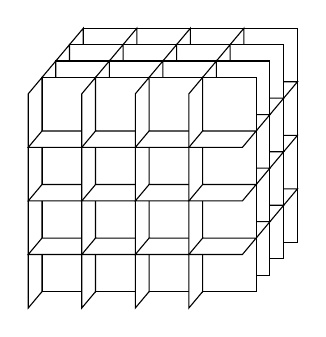
\begin{tikzpicture}[scale=0.68, z={(230:0.4cm)}]
                \foreach \z in {0, ..., 3} {
                    \ifthenelse{\z = 0}{}{
                        \filldraw[fill=white, draw=black] (0, 0, \z) -- ++(4, 0, 0) -- ++(0, 4, 0) -- ++(-4, 0, 0) -- cycle;
                    }
                    \foreach \x in {0, ..., 3} {
                        \ifthenelse{\x = 0}{}{
                            \filldraw[fill=white, draw=black] (\x, 0, \z) -- ++(0, 4, 0) -- ++(0, 0, 1) -- ++(0, -4, 0) -- cycle;
                        }
                        \foreach \y in {1, ..., 3} {
                            \filldraw[fill=white, draw=black] (\x, \y, \z) -- ++(1, 0, 0) -- ++(0, 0, 1) -- ++(-1, 0, 0) -- cycle;
                        }
                    }
                }
                \boxfront{0}{0}{0}{4}{4}{4}{dotted}
            \end{tikzpicture}
        \caption{Cuts.}
    \end{subfigure}
    \hfill
    \begin{subfigure}[b]{0.3\textwidth}
        \centering
            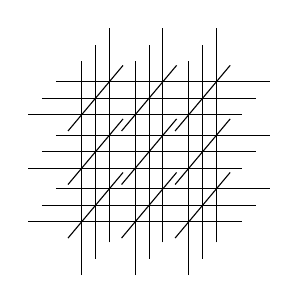
\begin{tikzpicture}[scale=0.68, z={(230:0.4cm)}]
                \boxback{0}{0}{0}{4}{4}{4}{dotted}
                \foreach \a in {1, ..., 3} {
                    \foreach \b in {1, ..., 3} {
                        \draw [black] (\a, \b, 0) -- ++(0, 0, 4);
                        \draw [black] (\a, 0, \b) -- ++(0, 4, 0);
                        \draw [black] (0, \a, \b) -- ++(4, 0, 0);
                    }
                }
                \boxfront{0}{0}{0}{4}{4}{4}{dotted}
            \end{tikzpicture}
        \caption{Grid lines.}
    \end{subfigure}
    \hfill
    \begin{subfigure}[b]{0.3\textwidth}
        \centering
            \begin{tikzpicture}[scale=0.68, z={(230:0.4cm)}]
                \boxback{0}{0}{0}{4}{4}{4}{dotted}
                \foreach \x in {1, ..., 3} {
                    \foreach \y in {1, ..., 3} {
                        \filldraw[black] (\x, 1, \y) circle (1pt);
                        \filldraw[black] (\x, 2, \y) circle (1pt);
                        \filldraw[black] (\x, 3, \y) circle (1pt);
                    }
                }
                \boxfront{0}{0}{0}{4}{4}{4}{dotted}
            \end{tikzpicture}
        \caption{Grid points.}
    \end{subfigure}
    \caption{Example of cuts and the grid of a cube in three dimensions.}
    \label{fig:grid}
\end{figure}

\begin{theorem}[Hoffman's grid theorem]\label[theorem]{thm:grid-theorem}
Suppose $d$ is a dimension tuple satisfying Hoffman's inequality and suppose $(B, C)$ is a packing of $d$ such that $B$ contains solely hyperrectangles. Then each hyperrectangle in $B$ contains exactly one grid point of the grid of $C$.
\end{theorem}

\begin{proof}
Let $d = \paren{x_1, x_2, \dotsc, x_n}$ and $s = x_1 + x_2 + \dotsb + x_n$. Assume without loss of generality that the packing has been translated, so that the anchor point of the surrounding hypercube is at the origin of the coordinate system, i.e.\ $C = (0, s)^n$, whereby we can reuse the grid construction described above.

We first show that every hyperrectangle in $B$ contains a grid point. Take some hyperrectangle $R$ in $B$ and write it as a Cartesian product $R = I_1 \times I_2 \times \dotsb \times I_n$ where each $I_i$ is a non-empty, open and bounded interval of $\R$. Next, pick some dimension $k$ in $\curly{1, 2, \dotsc, n}$. We would like to show that there exists a cut along the dimension $k$ which intersects the hyperrectangle $R$. Let $r_k$ denote the extent of the hyperrectangle $R$ along the $k$'th dimension, i.e.\ the width of the interval $I_k$. Since $(B, C)$ is a packing of $d$ the hyperrectangle $R$ is a subset of the hypercube $C$, whereby $I_k$ must be a subset of $(0, s)$. Notice that each $c_i$ from the grid construction is evenly distributed inside $(0, s)$ and cuts it up into $n + 1$ intervals of width equal to the cut distance $s/(n + 1)$. It then follows from Hoffman's inequality that $s/(n + 1) < x_1 \leq r_k$, so there must exist some $j_k$ in $\curly{1, 2, \dotsc, n}$ such that $c_{j_k}$ is in $I_k$. Then the cut $C_{k, j_k}$ at position $j_k$ along dimension $k$ must intersect the hyperrectangle $R$, since all $I_i$ are non-empty. Repeating this procedure for all dimensions $k$ gives $n$ cuts $C_{k, j_k}$ intersecting the hyperrectangle, one along each dimension. Intersecting these cuts results in a set with a single grid point, in this case $\paren{ c_{j_1}, c_{j_2}, \dotsc, c_{j_n} }$. This point is inside the hyperrectangle $R$, since each $c_{j_k}$ is inside$I_k$. Hence, there is a least one grid point inside each hyperrectangle in $B$.

Lastly, since $(B, C)$ is a packing of $d$, then the hyperrectangles in $B$ are pairwise non-overlapping. Then there can not be more than one grid point inside any of the $n^n$ hyperrectangles in $B$, since there are only $n^n$ grid points in total.
\end{proof}

\noindent Let us introduce a convenient way of working with this grid. Define the $n$-dimen\-sional grid point coordinates $G_n$ to be the set $\curly{1, 2, \dotsc, n}^n$ and note that for any $n$-dimensional hypercube, it is possible to identify each of its grid points through the bijective map from $G_n$ to the grid given by $\paren{p_1, p_2, \dotsc, p_n} \mapsto \paren{c_{p_1}, c_{p_2}, \dotsc, c_{p_n}}$. We will typically refer to a grid point by its coordinates\index{Grid point!coordinate} assigned via this bijection.

We say that two grid point coordinates are on the same \textit{grid line}\index{Grid line} if all but one of their entries match, and we say that this grid line runs along the dimension numbered by the index where the coordinates differ. Note that there are precisely $n$ grid point coordinates on any grid line. For each grid point coordinate $p$ in $G_n$ and each dimension $k = 1, 2, \dotsc, n$ we define $L(p, k, i)$ as the $i$'th grid point coordinate on the line passing through $p$ along dimension $k$ for $i = 1, 2, \dotsc, n$, that is
\[
L(p, k, i)_j =
\begin{cases}
i,   & \text{if } j = k \\
p_j, & \text{if } j \neq k
\end{cases}
\]
for $j = 1, 2, \dotsc, n$ and note that $L(p, k, p_k) = p$ for all $k = 1, 2, \dotsc, n$.

Suppose $d = \paren{x_1, x_2, \dotsc, x_n}$ is a dimension tuple satisfying Hoffman's inequality and suppose $(B, C)$ is a packing of $d$ such that $B$ contains solely hyperrectangles. Let $p$ be a grid point coordinate in $G_n$ and for $i = 1, 2, \dotsc, n$ define $w(p)_i$ as the extent along the $i$'th dimension of the hyperrectangle in $B$ containing this particular grid point. This is well-defined by Hoffman's grid theorem \labelcref{thm:grid-theorem}. We measure the \textit{stuffing}\index{Grid line!stuffing on} on a grid line $L(p, k, i)$ as the sum of the extents along the $k$'th dimension of the hyperrectangles associated with the grid points on the grid line, that is
\[
\sum_{i = 1}^n w(L(p, k, i))_k.
\]
A grid line is said to be \textit{completely stuffed}\index{Grid line!completely stuffed} if the stuffing on it equals the extent of the surrounding hypercube. With these notions we are ready to prove the next result, which is a generalization of Hoffman's proof of the three-dimensional case in \cite[p. 220]{Hoffman1981} and therefore named after him.

\begin{theorem}[Hoffman's line theorem]\label[theorem]{thm:line-theorem}
Suppose $d$ is a dimension tuple satisfying Hoffman's inequality and suppose $(B, C)$ is a packing of $d$ consisting solely of hyperrectangles. Then all grid lines are completely stuffed.
\end{theorem}

\begin{proof}
Notice that there are $n^n$ grid lines in total. We wish to measure the stuffing on each of these grid lines. Let $S$ denote the sum of stuffing on all of the $n^n$ grid lines.

By Hoffman's grid theorem \labelcref{thm:grid-theorem} each of the $n^n$ hyperrectangles contains precisely one grid point. Pick some grid point $p$, let $R_p$ be the hyperrectangle in $B$ containing $p$ and consider its dimension tuple $r = \paren{r_1, r_2, \dotsc, r_n}$. Let $s$ denote the sum of $d$ and observe that this dimension tuple must have the same sum as $r$. The grid point $p$ lies on exactly $n$ grid lines, one along each different dimension. Thus, the hyperrectangle $R_p$ will contribute with $r_i$ worth of stuffing to the grid line through $p$ along dimension $i$ for all $i = 1, 2, \dotsc, n$. Hence, $R_p$ contributes with a total of $s$ worth of stuffing to $S$. So does all of the $n^n$ hyperrectangle, whereby $n^n s \leq S$.

Furthermore, none of the $n^n$ grid lines can hold more than $s$ worth of stuffing without breaking some requirement of being a packing as specified in \cref{def:general-packing}. Thus, $S \leq n^n s$, so $S = n^n s$, whereby each grid line must have exactly $s$ worth of stuffing. Hence, all grid lines are completely stuffed.
\end{proof}

\noindent This result provides enough information to determine each of the hyperrectangles simply by knowing the dimension tuple of each hyperrectangle, since the only way to fit them inside the surrounding hypercube is by stacking them right next to each other. We can encode all of the information necessary to construct such a packing in a mapping assigning a permutation of $\curly{1, 2, \dotsc, n}$ to each grid point coordinate in $G_n$ specifying the dimension tuple (intuitively ``orientation'') of the hyperrectangle containing that particular grid point. Let $S_n$ be the set of permutations of $\curly{1, 2, \dotsc, n}$, that is bijections from the set to itself.

\pagebreak
\begin{definition}[Hoffman packing]\label[definition]{def:hoffman-packing}\index{Hoffman packing}
The map $P \colon G_n \to S_n$ is a \textit{Hoffman packing} of a dimension tuple $d = \paren{x_1, x_2, \dotsc, x_n}$ if the following procedure results in a packing $(B, C)$ of $d$. Let $s$ denote the sum of $d$ and let the surrounding hypercube $C = (0, s)^n$. For every grid point coordinate $p$ in $G_n$ place a hyperrectangle in $B$ with dimension tuple $w(p) = \paren{x_{\sigma(1)}, x_{\sigma(2)}, \dotsc, x_{\sigma(n)}}$ where $\sigma = P(p)$ and with anchor point $a(p)$ determined recursively for $i = 1, 2, \dotsc, n$ by
\[
a(p)_i = \begin{cases}
0 &                      \text{if } p_i = 1 \\
a(L(p, i, p_i - 1))_i + w(L(p, i, p_i - 1))_i & \text{otherwise}.
\end{cases}
\]
\end{definition}

\noindent Intuitively, $L(p, i, p_i - 1)$ is the grid point coordinate preceding $p$ on the grid line through $p$ along dimension $i$. This grid point coordinate exists as long as $1 < p_i \leq n$. The anchor point can also be stated explicitly for $i = 1, 2, \dotsc, n$ as
\[
a(p)_i = \sum_{k = 1}^{p_i - 1} w(L(p, i, k))_i.
\]
We say that $P$ \textit{produces}\index{Packing!produced by Hoffman packing} the packing $(B, C)$. It is possible to perform the above procedure for any map $P \colon G_n \to S_n$ and we will refer to the result as a \textit{pseudo-packing}\index{Packing!pseudo-}, since it does not necessarily satisfy the criteria in \cref{def:general-packing} of being a packing of $d$. For any grid point coordinate $p$ we will refer to the hyperrectangle $R_p$ with anchor-point $a(p)$ and dimension tuple $w(p)$ as the hyperrectangle \textit{associated}\index{Grid point!associated hyperrectangle} with $p$. Note that if the dimension tuple does not satisfy Hoffman's inequality, then the grid point $p$ need not be inside $R_p$. We will also refer to the right interval endpoints of $R_p$ as $b(p)$, i.e.\ $b(p) = a(p) + w(p)$.

Define two Hoffman packings of $d$ as \textit{equivalent}\index{Hoffman packing!equivalent} if they produce equivalent packings. We will refer to their equivalence class as a \textit{unique}\index{Hoffman packing!unique} Hoffman packing. At long last, it is possible to give meaning to a packing which is independent of the choice of dimension tuple.

\begin{definition}[Universal packing]\label[definition]{def:universal-packing}\index{Universal packing}
The map $P \colon G_n \to S_n$ is a \textit{universal packing} if it is a Hoffman packing of any dimension tuple satisfying Hoffman's inequality.
\end{definition}

\noindent This above definition restricts itself to dimension tuples satisfying Hoffman's inequality, but in \cref{sec:truely-universal-packing} we will discuss the possibility of using a universal packing to produce a packing of \textit{any} increasing dimension tuple.

\begin{remark}
When defining a Hoffman packing in \cref{def:hoffman-packing} we have restricted ourselves to packings consisting solely of hyperrectangles (i.e.\ general hyperrectangles which are in fact hyperrectangles). The primary reason for this restriction is that it turns the packing problem into a combinatorial problem. However, as the focus shifts from Hoffman packings to universal packings we can better justify this choice. A universal packing should in particular produce a packing of a dimension tuple of a hypercube, i.e.\ a dimension tuple $d = \paren{x_1, x_2, \dotsc, x_n}$ where $x_1 = x_2 = \dotsb = x_n$. In this case the AM-GM inequality is in fact an equality, so there can not be any unoccupied ``room'' in a packing of $d$. Intuitively, we can convince ourselves that this forces all of the hypercubes to be stacked snugly as \cref{fig:2d-packing-squares} illustrates in the two-dimensional case.
\end{remark}

\noindent We define two universal packings to be \textit{equivalent}\index{Universal packing!equivalent} if they produce equivalent packings for any dimension tuple satisfying Hoffman's inequality. We will refer to their equivalence class as a \textit{unique}\index{Universal packing!unique} universal packing. Finally, we are able to refine our question of how many different packings there are in a given dimension.

\begin{question}\label[question]{q:count}
How many unique universal packings are there in $n$ dimensions?
\end{question}
